\section{Introduction}  
\begin{figure}[H]  
	\centering  
	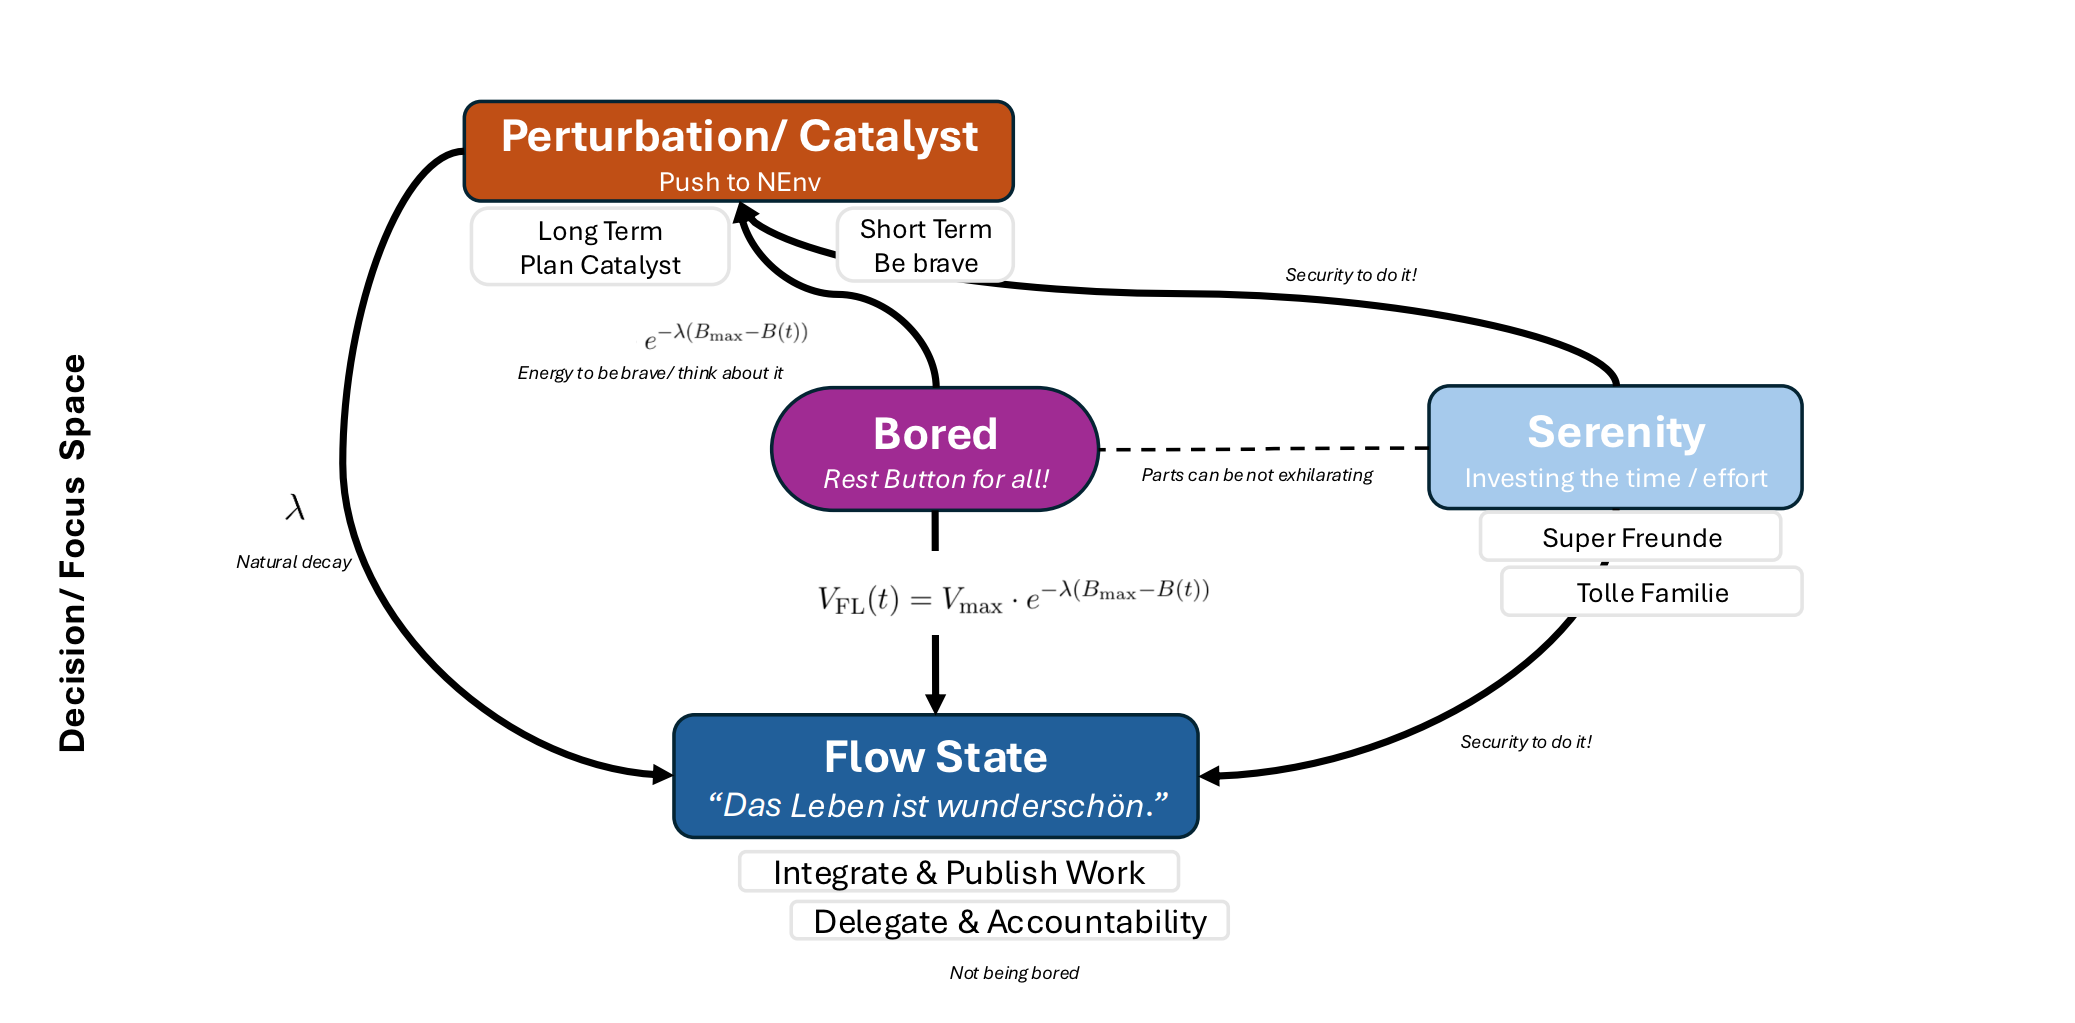
\includegraphics[scale=0.5]{attachment/chapter_OWN/DSci_Rubic__Personal_III}  
	\caption{Decision and Focus Space (Desired and Necessary Feelings)}  
\end{figure}  

With v3, the personal rubric becomes more focused on:  
\begin{itemize}  
\item A new, more conscious state: \textbf{Being bored} – as a way to reset myself.  
\item Identifying and initiating \textbf{catalytic events} that \textbf{perturb} my current environment.  
\end{itemize}  

Previously, the state \textit{Challenged} has been transformed into \textbf{Flow State}. This shift occurred to emphasize the feeling state rather than setting specific challenges—at least, not at this stage.\footnote{  
Certain aspects of the \textit{Serenity} state fulfill this role as well, particularly with \gls{p_NFM} and Franziska.  
}  

The \textit{flow state} is placed at the bottom because it requires less focus, as there is a natural gravitation toward it.  

On the other hand, \textit{Serenity} remains the key state to prioritize. While it is still central, it does not require as much focus at the moment. With the added responsibility of \gls{p_NFM}, the \textit{reset button} has become more important—where previously, it was not a priority.  

The aspect of \textit{being challenged} is still relevant but is now integrated differently within this framework.  

 

\section{Serenity and Flow State}
\begin{comment}
Die Überlegung dahinter ist, dass die Maximierung des stimulierenden Gefühls im Flow State (vorher: "Challenged") in Verbindung mit der Ausrichtung auf die Zukunft (Dopamin) keine langfristig tragfähige Basis für mich darstellt, da ich nicht auf die Zielsetzung für \textit{Serenity} verzichten möchte:

\begin{itemize}
    \item Eine großartige Familie
    \item und tolle Freunde.
\end{itemize}

Um das Gefühl der Herausforderung ohne größere Einbußen des allgemeinen Wohlbefindens zu erreichen, betrachte ich die Balance mit den Zielen für das Gefühl von \textit{Serenity} als essenziell.\\

Mir ist bewusst, dass einige Herausforderungen leichter zu bewältigen sind, wenn die gesetzten Ziele zurückgestellt oder aufgegeben werden. Meine Hoffnung und gleichzeitig meine selbst gesetzte Herausforderung ist es jedoch, einen Weg zu finden, Herausforderungen zu setzen und zu meistern, ohne dabei auf Familie und Freunde zu verzichten.
\end{comment}

The underlying consideration is that maximizing the stimulating feeling of the Flow State (previously: "Challenged") in combination with a future-oriented focus (dopamine) does not provide a sustainable long-term foundation for me, as I do not want to forgo my goals for 
\begin{itemize}
    \item A wonderful family
    \item and great friends.
\end{itemize}

To experience the feeling of challenge without major sacrifices to overall well-being, I see maintaining a balance with the goals for the feeling of \textit{Serenity} as essential.\\

I am aware that some challenges can be more easily achieved by postponing or abandoning set goals. However, my hope—and at the same time, my self-imposed challenge—is to find a way to set and accomplish challenges without having to sacrifice family and friendships.

\section{Perturbation}
\subsection{General Understanding}
% Simple -> Brilliant
% Color
%\definecolor{Rubric_gray}{RGB}{208,208,208}
%\definecolor{Rubric_FlowState_Lapis_Lazuli}{RGB}{33,95,154}
%\definecolor{Rubric_Pertubation_Rust}{RGB}{192,79,21}
%\definecolor{Rubric_Board_Violet}{RGB}{160,43,147}
%\definecolor{Rubric_Serentiy_BabyBlue}{RGB}{166,202,236}

Perturbing my current environment is essential for counteracting the decay of value, especially in the flow-state environments I inhabit.

For me, transitioning to new environments often requires a catalytic event rather than a slow, gradual shift. There is usually a barrier to overcome, and the natural gravitas of the flow state makes change difficult. Without a decisive disruption, adaptation tends to stagnate.

\subsection{Horizon: Catalytic Events}

In general, there should be only a few key topics within a given period that drive a push toward a new environment. The five-year horizon provides a better guide to identifying the desired perturbations. This yearly horizon focuses on what you actively commit your mind to.


\paragraph{This year}
\begin{figure}[H]  
	\centering  
\begin{tikzpicture}[scale=1.0]

% -----------------------------------------
% Serenity
%------------------------------------------

  \begin{scope}[shift={(-3,0)}]
    % Draw the inner circle (radius = 1.5)
    \fill[Rubric_Serentiy_BabyBlue] circle (1.5);
    %\shade[Rubric_circlegradient_Challenge_Pertubation] circle (1.5);

		% Center node text   
      \node at (0,0) [
      font  = \textstyleInside,
      align = center
    ]{Serenity};

    % {Start}{End}
    \arcarrow{180}{0}{NFM Eingewoehnung (Block Time)}{Rubric_gray}
  \end{scope}
  

% -----------------------------------------
% Pertubation: Study & Research
%----------------------------------------

\begin{scope}[shift={(3,0)}]
    % Draw the inner circle (radius = 1.5)
    \shade[Rubric_circlegradient_Challenge_Pertubation] circle (1.5);

		% Center node text   
      \node at (0,0) [
      font  = \textstyleInside,
      align = center
    ]{Study \\ Research};

    % Example arcs
    % Start at 0 End at 60
    \arcarrow{175}{0}{Keep deepen technical Knowledge}{Rubric_gray}
    \arcarrow{185}{355}{Own Research: (Block Time)}{Rubric_gray}

  \end{scope}
  

% -----------------------------------------
% Pertubation: Real Challenges
%----------------------------------------

\begin{scope}[shift={(0,5)}]
    % Draw the inner circle (radius = 1.5)
    \shade[Rubric_circlegradient_Challenge_Pertubation] circle (1.5);

		% Center node text   
      \node at (0,0) [
      font  = \textstyleInside,
      align = center
    ]{Real \\ Challenges};

    % {Start}{End}
    \arcarrow{185}{0}{Certified OFK Assessment Center (DB)}{Rubric_gray}
  \end{scope}


%-----------------------------------------
% Bored
%----------------------------------------

\begin{scope}[shift={(0,-5)}]
    % Draw the inner circle (radius = 1.5)
    \shade[Rubric_circlegradient_Bored_Perturbation] circle (1.5);

		% Center node text   
      \node at (0,0) [
      font  = \textstyleInside,
      align = center
    ]{Bored};

    % {Start}{End}
    \arcarrow{185}{0}{Reset Times (Single Days)}{Rubric_gray}
  \end{scope}

\end{tikzpicture}
\caption{Meilstones untill 20.12.2025}
\end{figure}



Technically, placing \textbf{NFM Moment* (Serenity)} as a push towards a new environment under perpetuation might be understood as intentionally pushing myself out of the \textit{flow state} to spend time with \gls{p_NFM}.

\paragraph{Current Five Years}

In general, there should be only a few key topics within a given period that drive a push toward a new environment. The five-year horizon provides a better guide to identifying the desired perturbations.

This timeline is a tool to align and assess capacity and to conduct an honest assessment of what is possible.

\begin{figure}[H]  
	\centering  
	%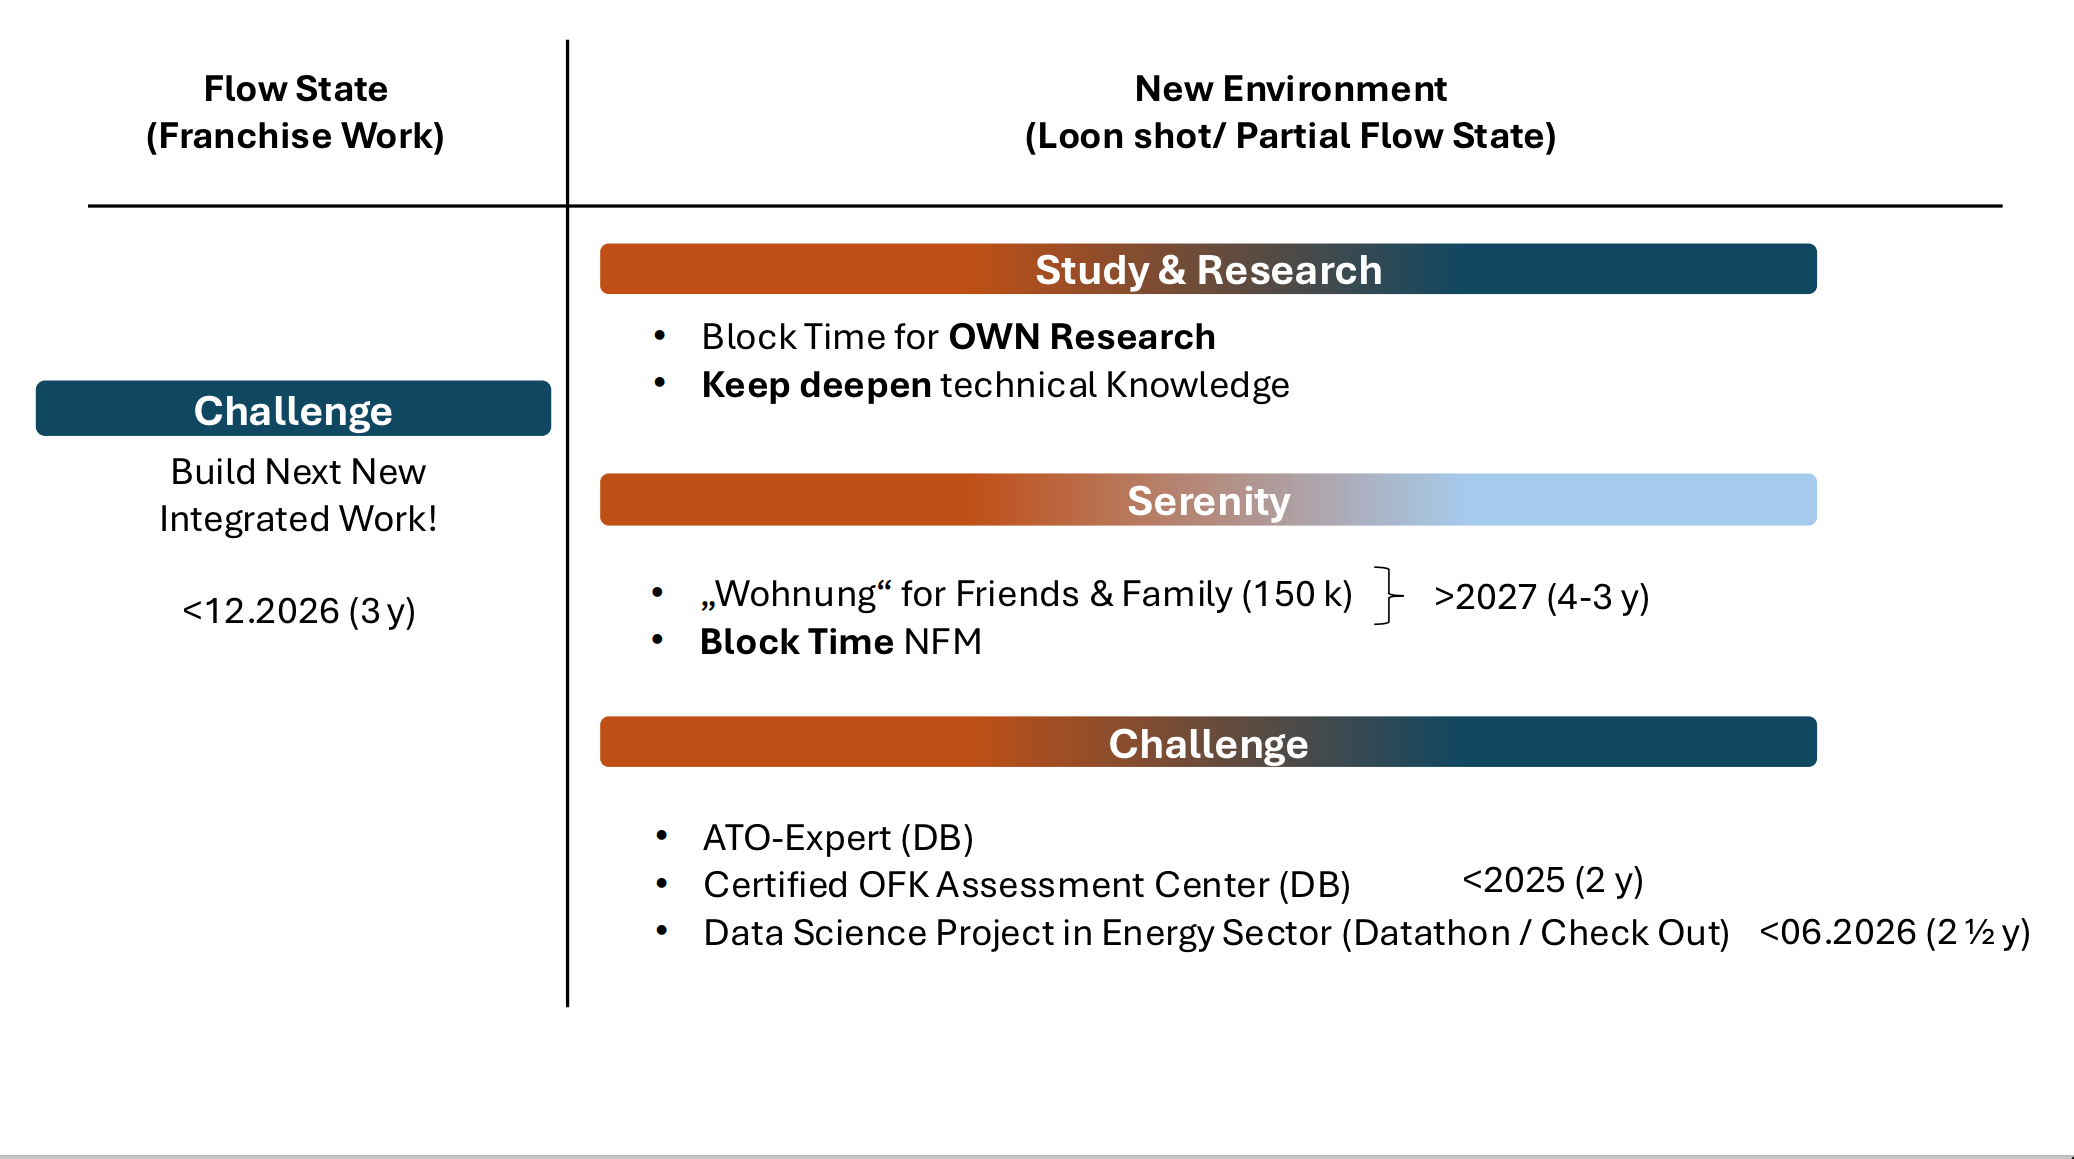
\includegraphics[scale=0.5]{attachment/chapter_OWN/Personal_Rubric__Timeline}
	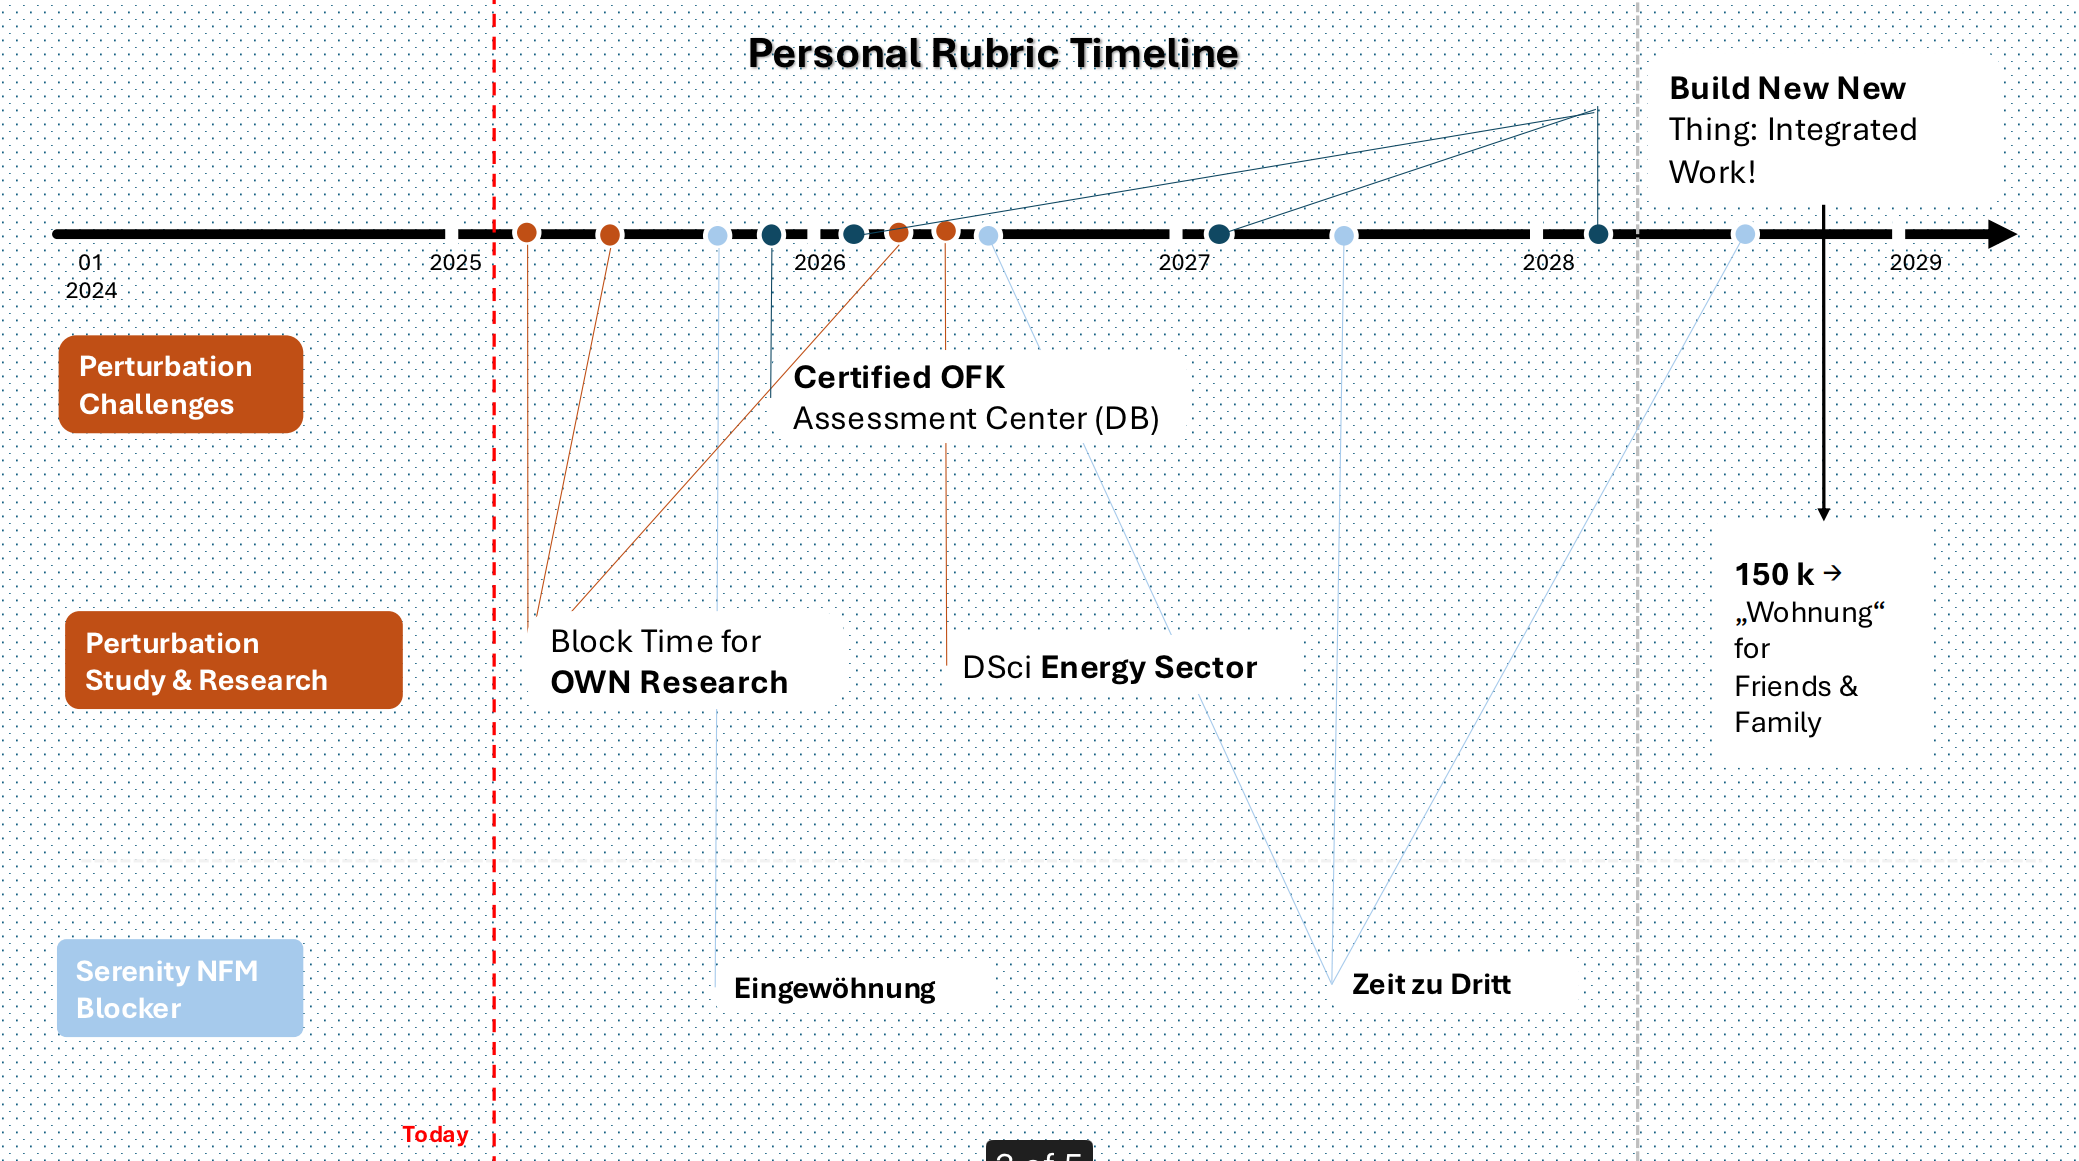
\includegraphics[scale=0.3]{attachment/chapter_OWN/Personal_Rubric__Timeline_II}
	\caption{Time line next five years}  
\end{figure}

\begin{figure}[H]  
	\centering  
\begin{tikzpicture}[scale=1.0]

% -----------------------------------------
% Pertubation
%------------------------------------------

  \begin{scope}[shift={(0,3)}]
    % Draw the inner circle (radius = 1.5)
    \fill[Rubric_Pertubation_Rust] circle (1.5);
    %\shade[Rubric_circlegradient_Challenge_Pertubation] circle (1.5);

		% Center node text   
      \node at (0,0) [
      font  = \textstyleInside,
      align = center
    ]{Pure\\ Pertubation};

    % {Start}{End}
    \arcarrow{190}{-29}{150k for Family  Friends (Social Growth)}{Rubric_gray}
  \end{scope}
  

% -----------------------------------------
% Challenges: But no pertubation!
%----------------------------------------

\begin{scope}[shift={(0,-3)}]
    % Draw the inner circle (radius = 1.5)
    \fill[gray] circle (1.5);

		% Center node text   
      \node at (0,0) [
      font  = \textstyleInside,
      align = center
    ]{Challenges};

    % Example arcs
    % Start at 0 End at 60
    \arcarrow{175}{0}{Build New New Thing}{Rubric_gray}

  \end{scope}
  


\end{tikzpicture}
\caption{Five Year Periode untill 31.12.2029}
\end{figure}

Why the color gray? This is because no perturbation of the current personal environment is necessary—just focus and work.

\begin{figure}[H]  
	\centering  
	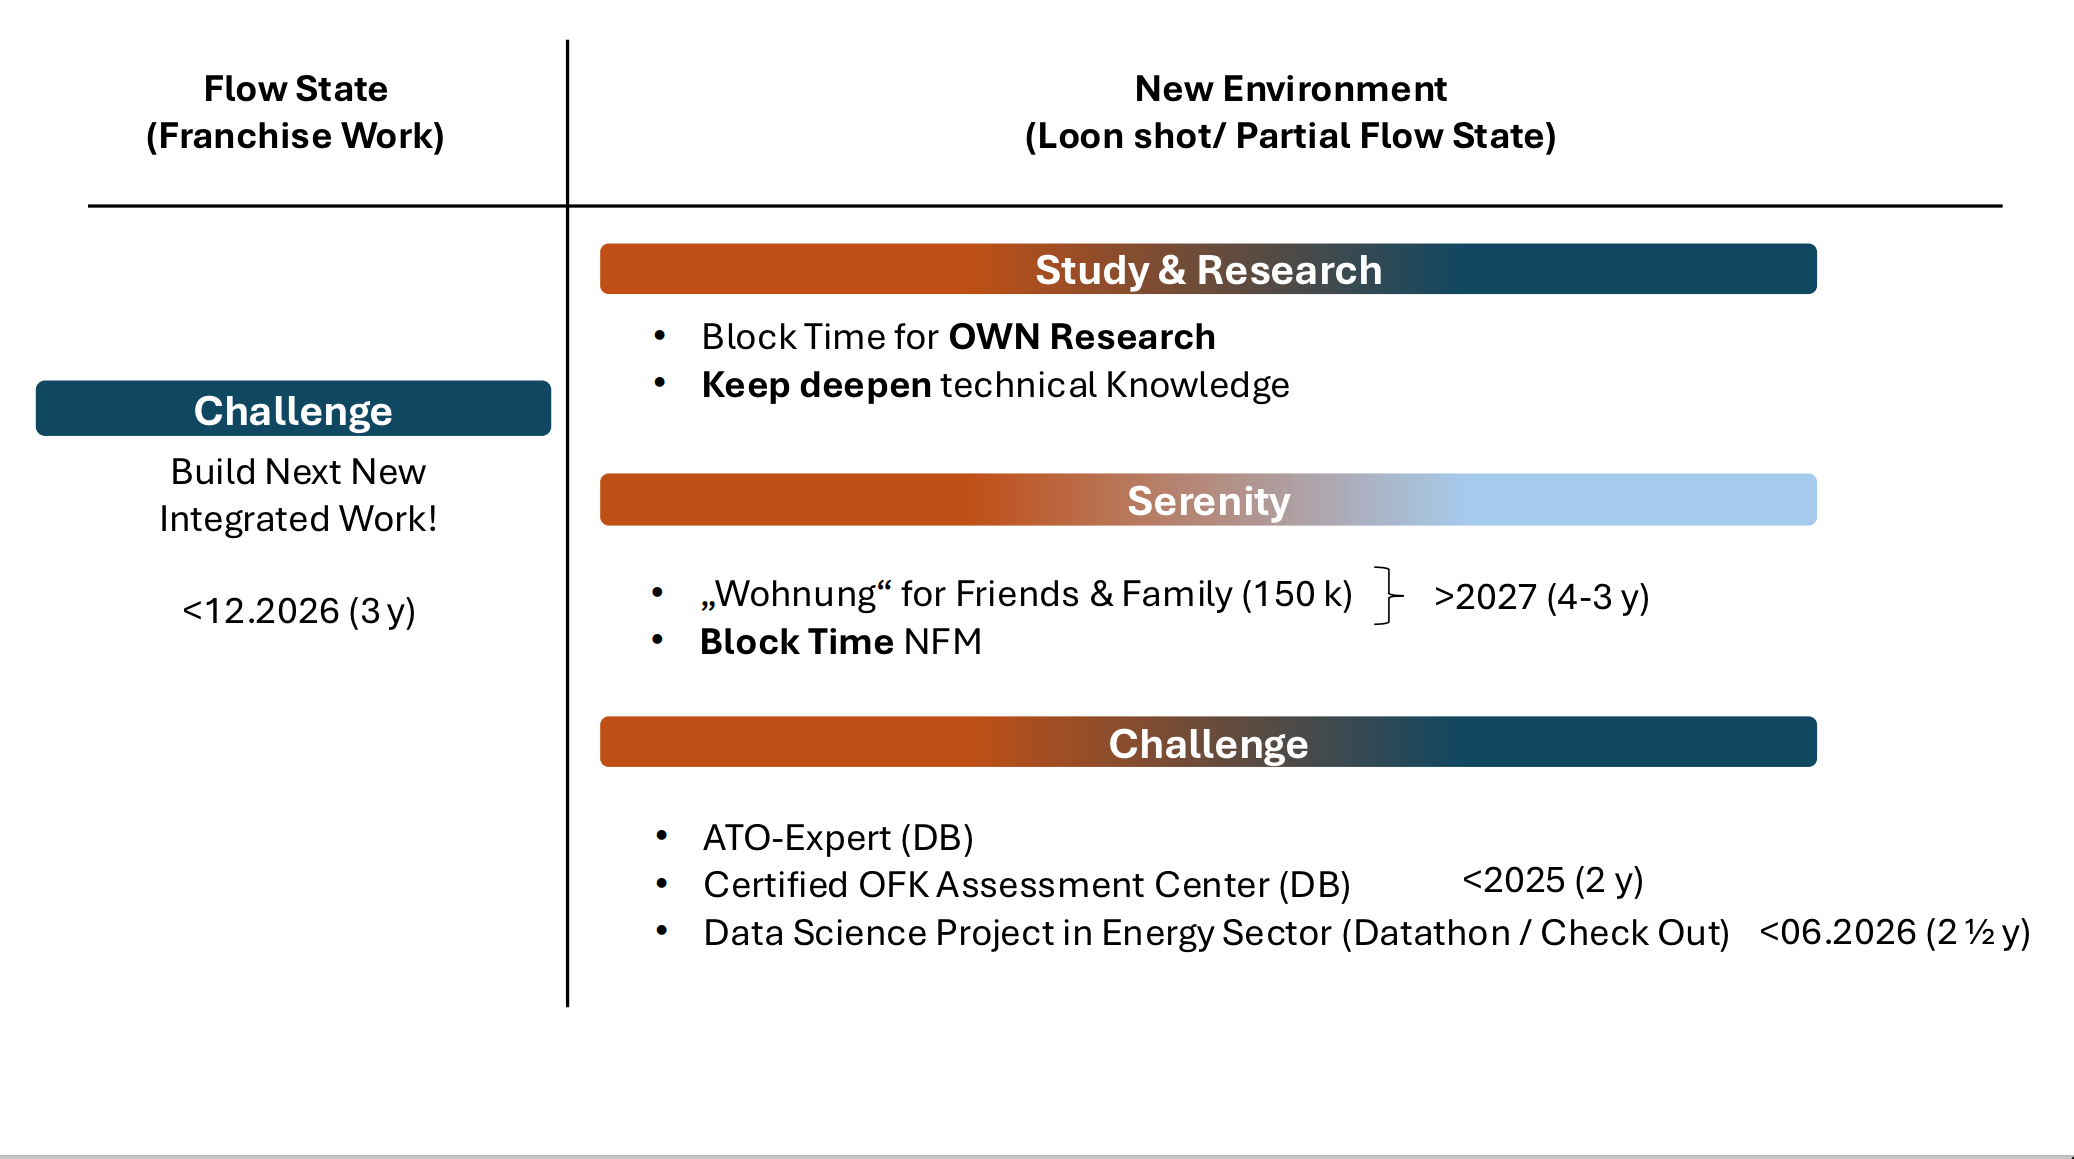
\includegraphics[scale=0.3]{attachment/chapter_OWN/Personal_Rubric__Timeline}
	%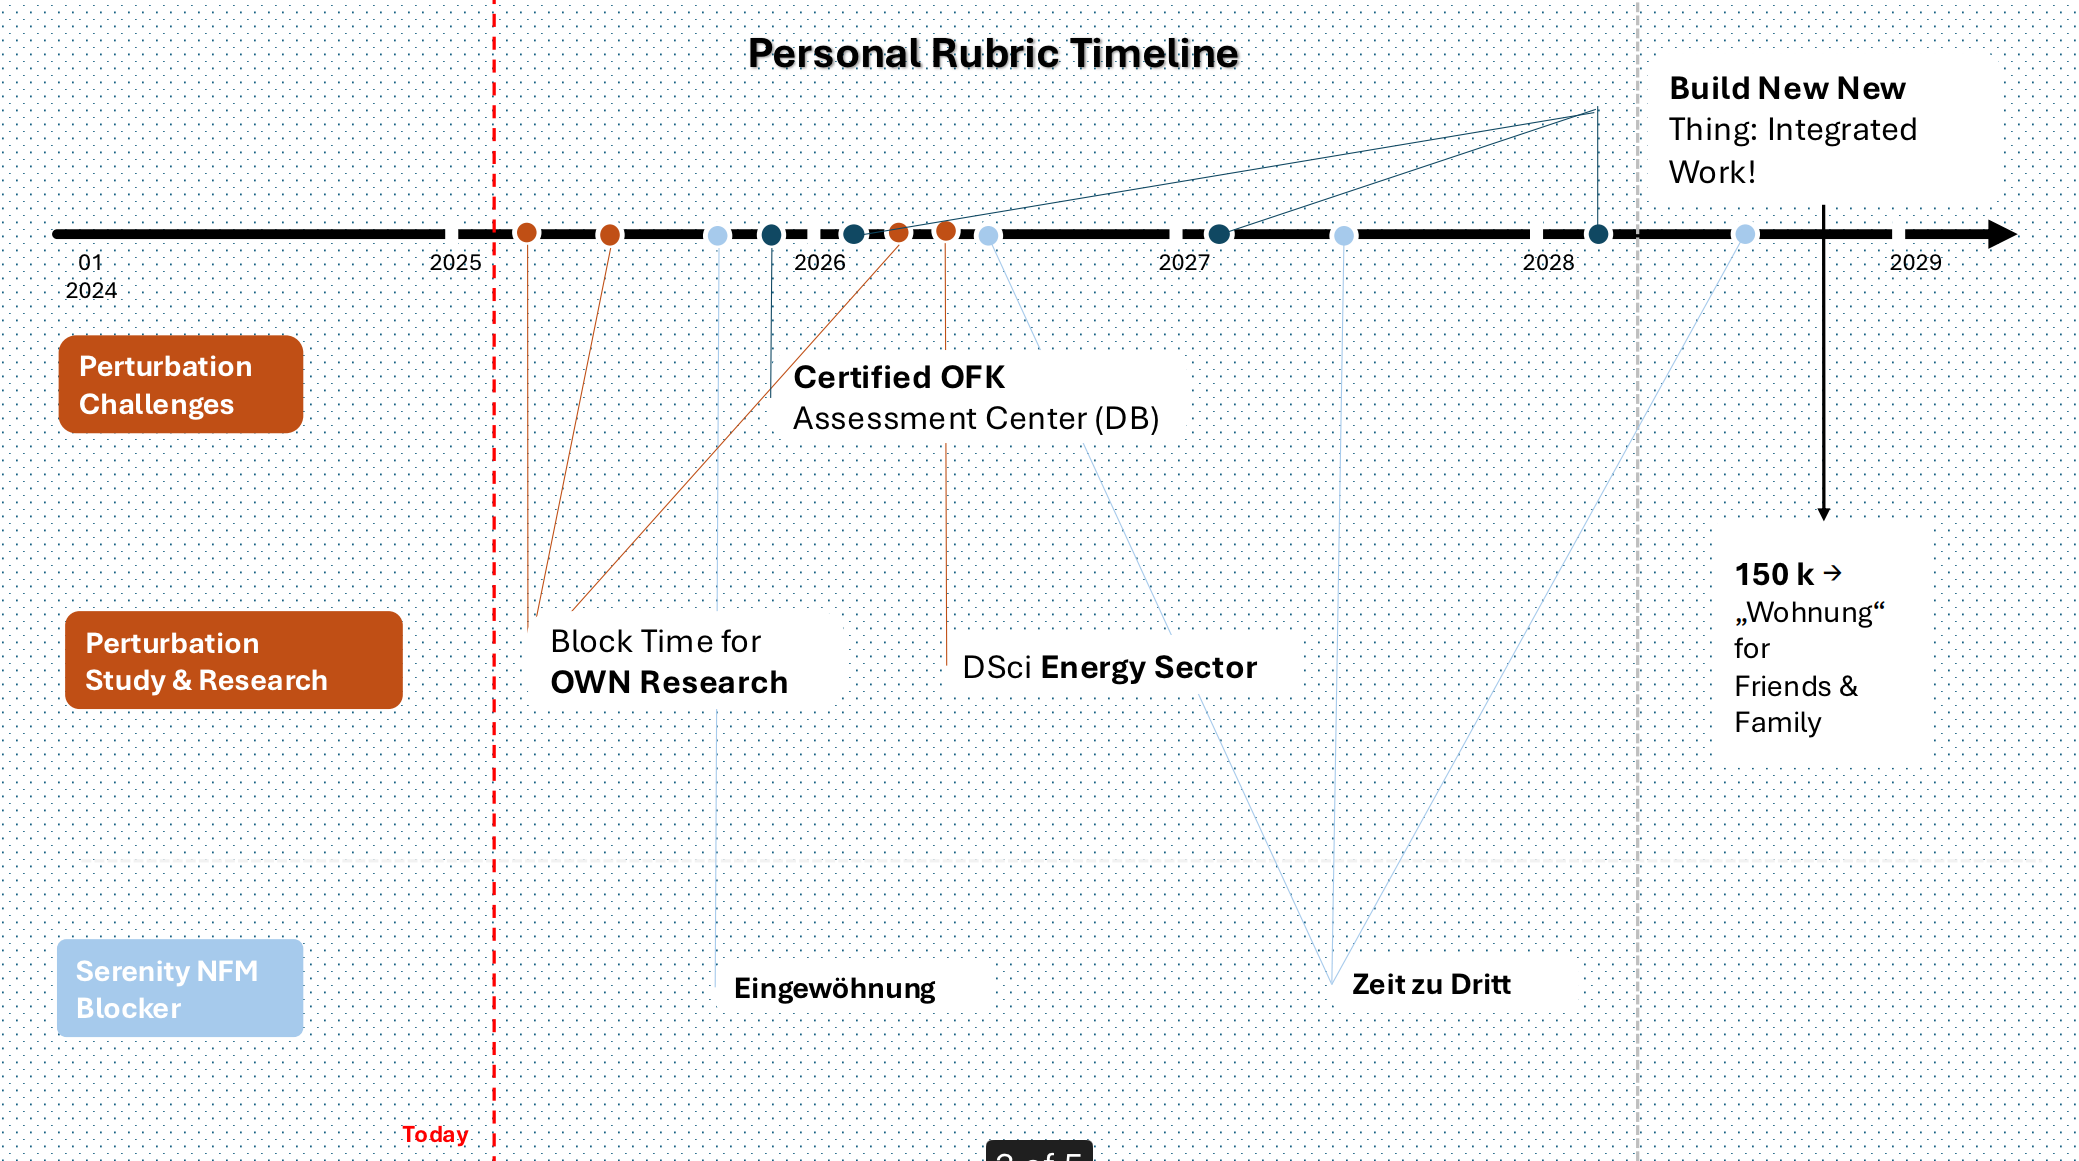
\includegraphics[scale=0.5]{attachment/chapter_OWN/Personal_Rubric__Timeline_II}
	\caption{Details: Time line next five years}  
\end{figure}

\paragraph{Longtermin: 20 Year Horizon Catalytic Events: 20 Years}

The push is that, during these periods, a jump into a new environment is required to sustain long-term growth and prevent decay. These five-year blocks are arbitrary intervals but serve to provide a long-term perspective, helping to clarify where you want to work towards.



\begin{figure}[H]  
	\centering  
\begin{tikzpicture}[remember picture, scale=0.8]
%\begin{tikzpicture}[remember picture, overlay, shift={(3,-1)}]

  % Define control points for the first S-shaped curve
  \coordinate (start) at (-4, 0);
  \coordinate (control1) at (6, -3);
  \coordinate (middle) at (0, -7);
  \coordinate (end1) at (-6, -11);

  % Draw the first S-shaped curve with color
  \draw[color= Rubric_FlowState_Lapis_Lazuli, thick] (start) .. controls (control1) .. (middle) .. controls (middle) and (end1) .. (end1);

  % Define control points for the second S-shaped curve
  \coordinate (control3) at (8, -2.5);
  \coordinate (middle2) at (4, -6.5);
  \coordinate (end2) at (-3, -14);

  % Draw the second S-shaped curve with color
  \draw[color= Rubric_Pertubation_Rust, thick] (start) .. controls (control3) .. (middle2) .. controls (middle2) and (end2) .. (end2);

  % General coordinates for arrow points
  \coordinate (arrow1) at ($(end1) + (-1, +1)$);
  \coordinate (arrow2) at ($(end2) + (+1, -1)$);
  \coordinate (arrow3) at ($(arrow2) + (-5.3, 0)$);

  % Draw the arrow head
  \draw (end1) -- (arrow1) -- (arrow3) -- (arrow2) -- (end2);

  % Shade the region between the two curves
  \begin{scope}
    \shade[bottom color= Rubric_FlowState_Lapis_Lazuli, top color= Rubric_FlowState_Lapis_Lazuli, opacity=0.8] 
      (arrow3) -- (arrow2) -- (end2) -- (middle2) .. controls (control3) .. (start) .. controls (control1) .. (middle) .. controls (middle) and (end1) .. (end1) -- (arrow1) -- (arrow3) -- cycle;
  \end{scope}

  % Draw and position the ovals corresponding to years
  \draw[color = red, fill = red, opacity = 0.8, line width=0.01cm] ($(start) + (0.806, -0.2)$) ellipse [x radius=0.15cm, y radius=0.03cm];
  \draw[color = black, fill = Rubric_Pertubation_Rust, opacity = 0.8, line width=0.01cm] ($(start) + (4.2, -1.074)$) ellipse [x radius=0.5cm, y radius=0.15cm];
  \draw[color = black, fill = Rubric_Pertubation_Rust, opacity = 0.8, line width=0.01cm] ($(start) + (6.85, -1.84)$) ellipse [x radius=0.75cm, y radius=0.3cm];
  \draw[color = black, fill = Rubric_Pertubation_Rust, opacity = 0.8, line width=0.01cm] ($(start) + (9.23, -3.55)$) ellipse [x radius=1.1cm, y radius=0.45cm];
  \draw[color = Rubric_Pertubation_Rust, fill = Rubric_Pertubation_Rust, opacity = 0.8, line width=0.01cm] ($(start) + (5.02, -7.7)$) ellipse [x radius=1.7cm, y radius=0.75cm];

  % Draw perpendicular dashed lines with fixed years
  \draw[color = red, dashed, opacity = 1] ($(start) + (0.806, -0.2)$) -- ++(90:3.5cm) 
    node[right, scale = 0.9, color = red] {2024};

	% Todays
  \draw[color = black, opacity = 1] ($(start) + (1.306, -0.35)$) -- ++(-90:1.75cm) 
    node[left, scale = 0.9, color = red] {TODAY (2025/ 02); 1 1/2y from 5 y};

 
    
  \draw[color = red, dashed, opacity = 1] ($(start) + (4.2, -1.074)$) -- ++(90:3.5cm) 
    node[right, scale = 0.9, color = orange] {2029};
  \draw[color = red, dashed, opacity = 1] ($(start) + (6.85, -1.84)$) -- ++(90:3.5cm) 
    node[right, scale = 0.9, color = yellow] {2034};
  \draw[color = red, dashed, opacity = 1] ($(start) + (9.23, -3.55)$) -- ++(-90:3.8cm)  
    node[right, scale = 0.9, color = green] {2039};
  \draw[color = red, dashed, opacity = 1] ($(start) + (5.02, -7.7)$) -- ++(-90:4.5cm) 
    node[right, scale = 0.9, color = Rubric_Pertubation_Rust] {2044};

  % Add text under the years
  \node[right, color = black, scale = 1.5] (1) at ($(start) + (0.87, -0.2)  + (90:2.8cm)$) {2024};
  \node[right, color = black, scale = 1] (2) at ($(start) + (0.87, -0.32)  + (90:2.4cm)$){Job Change} ;
  \node[right, color = black, scale = 1.5] (3) at ($(start) + (4.27, -1.074)  + (90:2.8cm)$) {5 years};
  \node[right, color = black, scale = 1] (4) at ($(start) + (4.27, -1.074) + (90:2.4cm)$){are over!} ;
  \node[right, color = black, scale = 1.5] (5) at ($(start) + (6.95, -1.84) + (90:2.8cm)$) {10 years};
  \node[right, color = black, scale = 1] (6) at ($(start) + (6.95, -1.84)+ (90:2.4cm)$) {are over!};
  \node[right, color = black, scale = 1] (7) at ($(start) + (6.95, -1.84) + (90:2cm)$) {amet};

  % Add text boxes for 2040 and 2045
  \node[right, color = black, scale = 1.5] (8) at ($(start) + (9.3, -3.55) + (-90:2.8cm)$) {15 years};
  \node[right, color = black, scale = 1] (9) at ($(start) + (9.3, -3.55) + (-90:3.2cm)$){are over!} ;
  \node[right, color = black, scale = 1.5] (10) at ($(start) + (5.2, -7.7) + (-90:3.4cm)$) {20 Years};
  \node[right, color = black, scale = 1] (11) at ($(start) + (5.2, -7.7) + (-90:3.8cm)$){are over!} ;

  % Draw boxes around the text nodes
  \node[draw, line width = 0.005cm, rounded corners, scale = 0.85, fit={(1) (2)}] {};
  \node[draw, line width = 0.005cm, rounded corners, scale = 0.85, fit={(3) (4)}] {};
  \node[draw, line width = 0.005cm, rounded corners, scale = 0.85, fit={(5) (6) (7)}] {};
  \node[draw, line width = 0.005cm, rounded corners, scale = 0.85, fit={(8) (9)}] {};  % Box for 2040
  \node[draw, line width = 0.005cm, rounded corners, scale = 0.85, fit={(10) (11)}] {}; % Box for 2045
\end{tikzpicture}
\end{figure}



\section*{Being Board - Flow State (Decay Model for Fun)}
We aim to model the daily value of my  Flow state I'm in, $ V_{\text{FL}}(t) $, which decays over time based on the behavior of $ B(t) $ - Boring. The behavior of $ B(t) $ is characterized by:
\begin{itemize}
    \item \textbf{Exponential decrease with latency:} $ B(t) $ decreases slowly during a latency period and then decays faster after the latency period ends.
    \item \textbf{Reset behavior:} $ B(t) $ is reset to $ B_{\text{max}} $ periodically after reaching a lower threshold (e.g., $ B(t) \to 0 $).
\end{itemize}

The decay of $ V_{\text{FL}}(t) $ is governed by $ B(t) $, such that as $ B(t) $ decreases, $ V_{\text{FL}}(t) $ decreases exponentially. If I'm highly board, the value of the flow state I can be in is the highest, if I was board the most.

\paragraph{Visualization}
The behavior is visualized as follows:
\begin{itemize}
    \item $ B(t) $: Decreases slowly during the latency period, then decreases faster after the latency period. Resets periodically to $ B_{\text{max}} $.
    \item $ V_{\text{FL}}(t) $: Decays exponentially in response to $ B(t) $, resetting to $ V_{\text{max}} $ whenever $ B(t) $ resets.
\end{itemize}

\begin{figure}[H]
	\centering
	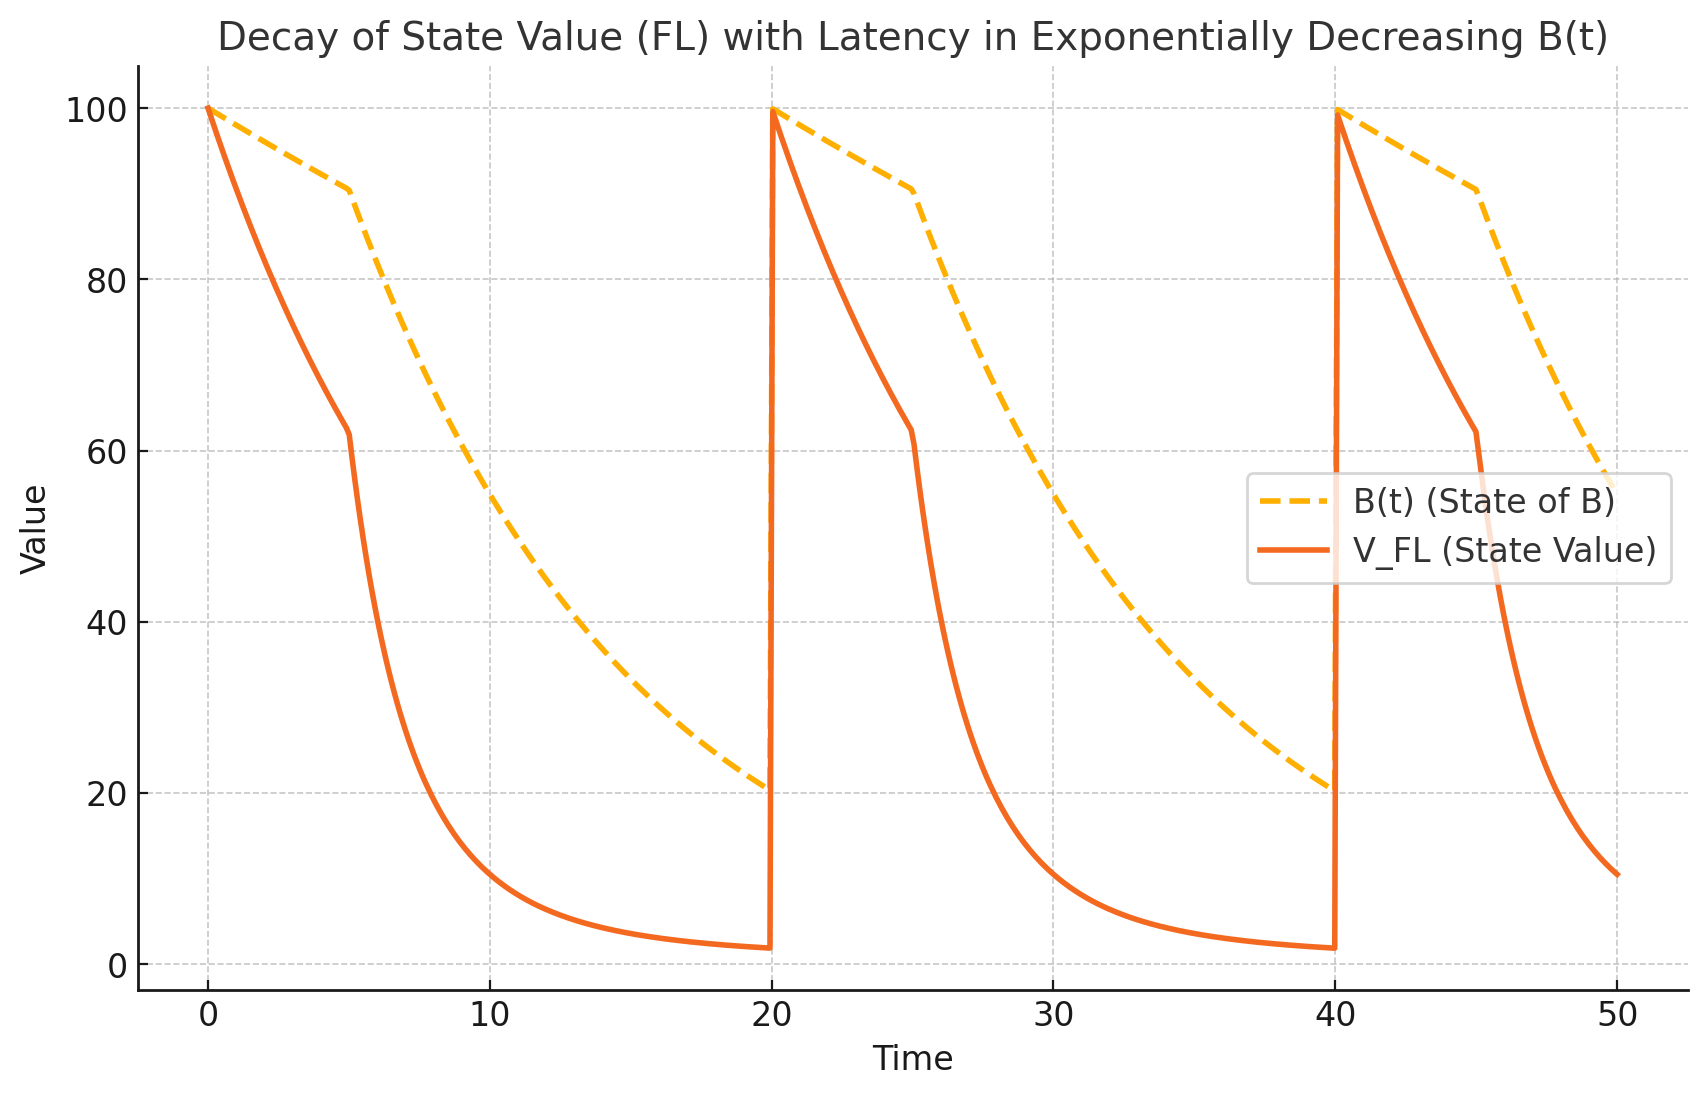
\includegraphics[scale = 0.5]{attachment/chapter_OWN/PRubric_Decay}
	\caption{Desired and necessary feelings}
\end{figure}



\paragraph{Modeling $ B(t) $: Exponentially Decreasing with Latency}
The function $ B(t) $ is modeled as a piecewise exponential decay:
\[
B(t) =
\begin{cases}
B_{\text{max}} \cdot e^{-\alpha t}, & \text{if } t \leq t_{\text{latency}}, \\
B_{\text{max}} \cdot e^{-\alpha t_{\text{latency}}} \cdot e^{-\beta (t - t_{\text{latency}})}, & \text{if } t > t_{\text{latency}},
\end{cases}
\]
where:
\begin{itemize}
    \item $ B_{\text{max}} $: Maximum value of $ B(t) $ when reset.
    \item $ \alpha $: Decay rate during the latency period (slow rate of decrease).
    \item $ \beta $: Decay rate after the latency period (faster rate of decrease).
    \item $ t_{\text{latency}} $: Duration of the latency period.
\end{itemize}

\paragraph{Modeling $ V_{\text{FL}}(t) $: Exponential Decay of State Value}
The state value $ V_{\text{FL}}(t) $ decays exponentially as $ B(t) $ decreases. It is given by:
\[
V_{\text{FL}}(t) = V_{\text{max}} \cdot e^{-\lambda (B_{\text{max}} - B(t))},
\]
where:
\begin{itemize}
    \item $ V_{\text{FL}}(t) $: Value of the state FL at time $ t $.
    \item $ V_{\text{max}} $: Maximum possible value of $ V_{\text{FL}}(t) $.
    \item $ \lambda $: Decay constant for $ V_{\text{FL}}(t) $.
\end{itemize}

\paragraph{Reset Behavior}
\begin{itemize}
    \item $ B(t) $ resets to $ B_{\text{max}} $ after reaching a threshold (e.g., $ B(t) \to 0 $), periodically every $ T_{\text{reset}} $ seconds.
    \item This causes $ V_{\text{FL}}(t) $ to restart from its maximum possible value, $ V_{\text{max}} $, after each reset.
\end{itemize}

\paragraph{Complete Behavior}
Combining these equations:
\begin{enumerate}
    \item For $ B(t) $:
    \[
    B(t) =
    \begin{cases}
    B_{\text{max}} \cdot e^{-\alpha t}, & t \leq t_{\text{latency}}, \\
    B_{\text{max}} \cdot e^{-\alpha t_{\text{latency}}} \cdot e^{-\beta (t - t_{\text{latency}})}, & t > t_{\text{latency}},
    \end{cases}
    \]
    where $ t $ resets to $ 0 $ after $ T_{\text{reset}} $.
    \item For $ V_{\text{FL}}(t) $:
    \[
    V_{\text{FL}}(t) = V_{\text{max}} \cdot e^{-\lambda (B_{\text{max}} - B(t))}.
    \]
\end{enumerate}



%%%%%%
\textit{I'm came with abilities and an emotional imprint.}

I can build up domain knowdledge an update this, to combine with my concitive abilities. How ever, think about how I feel, how I want to feel and how I may need to change how I feel, in order to satifice my core imprint, this the goal for this - Homostatice

I can't do much about the former, except build better prediction models for my self and a cummilate knowledge - but even this is limited. The later however, is more malible, or at least essesing it.